\documentclass[tikz,border=2]{standalone}
\usepackage{amssymb}
\usetikzlibrary{shadows,arrows,shapes,positioning,calc,backgrounds,fit}
\begin{document}
%%%%%%%%%%%%%%%%%%%%%%%%%%%%%%%%%%%%%%%
% colors
\definecolor{myBlue}{HTML}{0060AD}
\definecolor{myRed}{HTML}{DD181F}
%%%%%%%%%%%%%%%%%%%%%%%%%%%%%%%%%%%%%%%

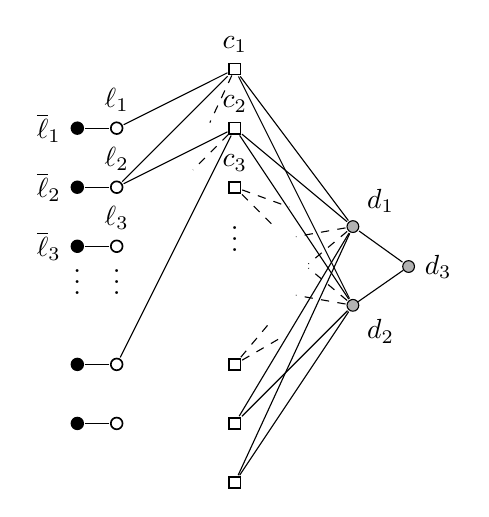
\begin{tikzpicture}
[scale=1,transform shape,
node distance=1cm,
%
vertex/.style={shape=circle,draw=black,inner sep=2pt,semithick},
clause/.style={shape=rectangle,draw=black,inner sep=2pt,semithick},
literal/.style={shape=circle,draw=black,inner sep=1.5pt,semithick},
nliteral/.style={literal,fill=black},
dummy/.style={literal,fill=black!30,thin},
%
edge/.style={draw,shorten >=.4pt,shorten <=.4pt},
dedge/.style={gray,>=latex', shorten >=.0pt, shorten <=.0pt, thick}]
%
%% clauses
\def\sep{0.75}
\begin{scope}
\foreach \x in {1,...,3}
\node (c\x) [clause,label=above:$c_\x$] at (0,-\sep*\x) {};
%% \node at (0,2.1) {$\vdots$};
\node at (0,-2.8) {$\vdots$};
\foreach \x in {6,...,8}
\node (c\x) [clause] at (0,-\sep*\x) {};
\end{scope}
%
%% literals
\begin{scope}[shift={(-1.5,-.75)}]
\foreach \x in {1,...,3}
\node (l\x) [literal,label=above:$\ell_\x$] at (0,-\sep*\x) {};
\node at (0,-2.6) {$\vdots$};
\foreach \x in {5,...,6}
\node (l\x) [literal] at (0,-\sep*\x) {};
\end{scope}
%
%% edges between clauses and literals
\draw[edge] (c1) -- (l1);
\draw[edge] (c1) -- (l2);
\draw[dashed] (c1) -- +(-115:.75);
%%
\draw[edge] (c2) -- (l2);
\draw[edge] (c2) -- (l5);
\draw[dashed] (c2) -- +(-135:.75);
%%
%% negative literals
\begin{scope}[shift={(-2,-.75)}]
\foreach \x in {1,...,3}
\node (nl\x) [nliteral,label=left:$\overline{\ell}_\x$] at (0,-\sep*\x) {};
\node at (0,-2.6) {$\vdots$};
\foreach \x in {5,...,6}
\node (nl\x) [nliteral] at (0,-\sep*\x) {};
\end{scope}
%
%% edges between lit and neg lit
\foreach \x in {1,...,3,5,6}
\draw[edge] (nl\x) -- (l\x);
%%
%% dummy variables
\begin{scope}[shift={(1.5,-2.75)}]
   \node (d1) [dummy,label=above right:$d_1$] {};
   \node (d2) [dummy,below of=d1,label=below right:$d_2$] {};
   \node (d3) [dummy,below right of=d1,label=right:$d_3$,shift={(0,.2)}] {};
\end{scope}
%%
%% edges between dummies
\draw[edge] (d2) -- (d3) -- (d1);
%%
%% edges between clauses and dummies
\draw[edge] (c1) -- (d1);
\draw[edge] (c2) -- (d1);
%% \draw[edge] (c3) -- (d1);
%% \draw[edge] (c6) -- (d1);
\draw[edge] (c7) -- (d1);
\draw[edge] (c8) -- (d1);
\draw[edge,dashed] (c3) -- +(-20:.75);
\draw[edge,dashed] (c3) -- +(-45:.75);
\draw[edge,dashed] (d1) -- +(190:.75);
\draw[edge,dashed] (d1) -- +(220:.75);
%%
\draw[edge] (c1) -- (d2);
\draw[edge] (c2) -- (d2);
%% \draw[edge] (c3) -- (d2);
%% \draw[edge] (c6) -- (d2);
\draw[edge] (c7) -- (d2);
\draw[edge] (c8) -- (d2);
\draw[edge,dashed] (c6) -- +(30:.75);
\draw[edge,dashed] (c6) -- +(50:.75);
\draw[edge,dashed] (d2) -- +(170:.75);
\draw[edge,dashed] (d2) -- +(140:.75);
%%
%% \begin{pgfonlayer}{background}
%% \node[fill=black!20,ellipse,minimum width=1cm,fit=(a2)(a6),label=above:$\overline{H}$]{};
%% \end{pgfonlayer}
%% % edges
%% \path
%% (.6,1.75) edge (1.5,1.25)
%% (.6,1) edge (1.5,1.5)
%% (.6,1.25) edge (1.5,2)
%% (.6,2) edge (1.5,2.5)
%% (.6,2.5) edge (1.5,2.75)
%% (.6,3) edge (1.5,2.25);
%% \node at (1.1,2.1) {$\vdots$};
%% %
%% \draw[->,dedge] (a7) -- ++(.5,.5) node [right,black] {\small degree $\leqslant h$};
%% \node [right] at (2.2,2) {$\Bigg\}$ {\small $h$ nodes}};
\end{tikzpicture}
{}
\end{document}
